\documentclass[12pt]{extarticle}
\usepackage[brazil]{babel}
\usepackage{graphicx, hyperref}
\usepackage{framed}
\usepackage[normalem]{ulem}
\usepackage{amsmath}
\usepackage{amsthm}
\usepackage{amssymb}
\usepackage{amsfonts}
\usepackage{enumerate}
\usepackage[utf8]{inputenc}
\usepackage[top=1 in,bottom=1in, left=1 in, right=1 in]{geometry}
\usepackage{graphicx}
\usepackage[skip=2pt]{caption}
\usepackage{blindtext}
\usepackage[fixlanguage]{babelbib}
\usepackage[alf]{abntex2cite}
\bibliographystyle{abntex2-alf}
\captionsetup{font={small}} 
\graphicspath{{Figuras/}}
\usepackage{appendix}
\newcommand{\asp}[1]{``#1"}
\usepackage[colorinlistoftodos]{todonotes}
\newcommand{\nota}[1]{\todo[color=black!10, bordercolor=white!100, linecolor = black!20, size =\scriptsize]{#1} }
\definecolor{mypink1}{rgb}{0.858, 0.188, 0.478}
\definecolor{mypink2}{RGB}{219, 48, 122}
\definecolor{mypink3}{cmyk}{0, 0.7808, 0.4429, 0.1412}
\definecolor{mygray}{gray}{0.6}
\newcommand{\arb}{um elemento arbitrário }
\newenvironment{resposta}{ \color{mygray}}{}
\newcommand{\true}{\textcolor{red}{\textbf{\textit{V}}}}
\newcommand{\false}{\textcolor{red}{\textbf{\textit{F}}}}
\newcommand{\keys}[1]{\{#1\}}
\newenvironment{direta}{}{
\begin{flushright}
    Q.E.D
\end{flushright}
}
\newenvironment{contradicao}{A prova é por contradição.}{
\begin{flushright}
    Q.E.D
\end{flushright}
}
\newenvironment{contrapositiva}{A prova é pela contrapositiva.}{
\begin{flushright}
    Q.E.D
\end{flushright}
}
\newcommand{\definition}[3][x]{\{#1|#1 \in \mathbb{#2},#3\}}
\newcommand{\natura}{\mathbb{N}}
\newcommand{\integer}{\mathbb{Z}}
\newcommand{\real}{\mathbb{R}}
\newenvironment{pif}[3][1]{
Tomando $n = #1$ então $#2$ e $#3$

Agora vamos assumir que a expressão é valida para $#1 > n \leq k$ e vamos provar que funciona para $n=k+1$.
}{}
\newcommand{\arranjo}[2]{A_{#1,#2}=\frac{#1!}{(#1-#2)!}}
\newcommand{\arranjoform}[2]{\frac{#1!}{(#1-#2)!}}
\newcommand{\conbination}[2]{C_{#1,#2}=\frac{#1!}{#2!(#1-#2)!}}
\newcommand{\conbinationform}[2]{\frac{#1!}{#2!(#1-#2)!}}
\newcommand{\rconbination}[2]{CR_{#1,#2}=\frac{(#1+#2-1)!}{#2!(#1-1)!}}
\newcommand{\clinear}[1]{\foreach \i in {1,...,#1}{x_\i+}}
\newcommand{\fatorial}[2]{\foreach \i in {#1,...,#2}{\i.}}
\newcommand{\soma}[2]{\sum_{n=#1}^{\infty}#2}
\newcommand{\texto}{\color{mygray}\blindtext\color{black}}



%--------------%--------------%----------------------%-----------%--------------

\title{Projeto Wikiaves (WAV) x SpeciesLink (SLI)}
\author{Universidade Federal do ABC}
\date{Janeiro, 2021}

\begin{document}


\maketitle

\textbf{Considerações}
\begin{enumerate}
\item 
\end{enumerate}
\newpage

\section{Análise Univariada}

\hrulefill



\hrulefill


\begin{resposta}
Os sítios Wikiaves e SpeciesLink são bases de dados distintas que contam com registros de espécies de aves. No estado de São Paulo, a capacidade amostral varia de acordo com sítio analisado, o Wikiaves, cobre 631 dentre os 645 municípios do estado e, o SpeciesLink, cobre 174. Ao valer-se apenas dos municípios registrados em ambas as bases de dados, há apenas uma que aparece exclusivamente no SpeciesLink, esta cidade, por sua vez, não possuí grande influência sob os valores restantes da amostra. 

Por este motivo as análises conduzidas se dividirão em 3 categorias: Wikiaves, SpeciesLink e Wikiaves valendo-se apenas dos 173 municípios que possuem registros em ambas as bases.

\end{resposta}

\begin{figure}[h!]
\centering
{\scriptsize Tabela 1: Número de municípios amostrados, registros e espécies nos bancos de dados: WAV = Wikiaves, SLI = SpeciesLink, WAV2 = WAV com municípios redundantes em SLI.}
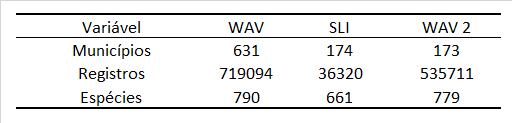
\includegraphics{Imagens/T01.png}
\end{figure}

\begin{resposta}
Em sequencia, serão abordadas as variáveis de registros por município, espécies por município e registros por espécie.
\end{resposta}

\subsection{Registros por Município}

\begin{resposta}
As medidas de tendencia central e dispersão para o número de registros por município encontram-se na tabela a seguir: 
\end{resposta}

\begin{figure}[h!]
\centering
{\scriptsize Tabela 2: Estatísticas de tendência central e dispersão para o número de registros por município em cada banco de dados: WAV = Wikiaves, SLI = SpeciesLink, WAV2 = WAV com municípios redundantes em SLI. Valores de média (m) e desvio-padrão (dp) em Log10 foram retrotransformados (Retro). min-max = valores extremos, q1-q3 = quartis.}
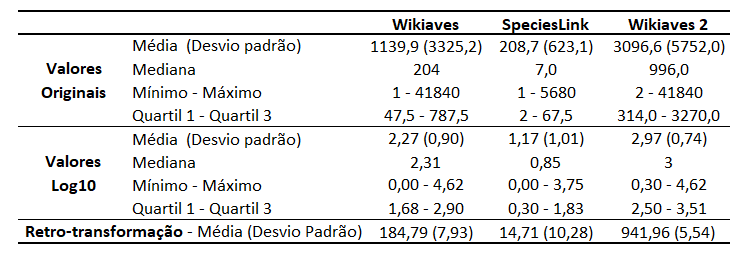
\includegraphics{Imagens/T02.png}
\end{figure}

\newpage

\begin{resposta}
A quantidade de registros no Wikiaves é uma ordem de grandeza maior que a do SpeciesLink. Embora as disparidades não sejam tão evidentes, a média de registro por município acompanha este padrão. Entretanto, esse tópico traz uma mediana que é, no mínimo, cinco vezes menor que a média para ambas as bases analisadas, este fato, acrescido das distâncias distintas entre os quartis justificam o desvio padrão, que vale cerca de três vezes a média. Isto sugere que a distribuição de registros por município não é homogenia quando exploradas as variáveis originais. Para que os valores sejam significativos, aplica-se uma transformação logarítmica cujos valores estão, igualmente, dispostos na tabela. A desproporção entre as médias dos bancos de dados é maior na relação SpeciesLink - Wikiaves 2, também este possui cerca de quatorze vezes a quantidade de registros por município que o SpeciesLink. Quando analisados os quartis, a disparidade entre os sítios aumenta, bem como para a mediana. 

Após a transformação, percebe-se que os valores para o SpeciesLink permanecem não uniformes, contudo, mais uniformes que anteriormente. O Wikiaves, por outro lado, apresenta-se de forma quase homogenia, a distância entre a média e a mediana é de 0,16, isso representaria 1,44 em valores não logarítmicos, contrastando com a distância de 935,6 obtida pelas variáveis originais, ademais, o desvio padrão neste sítio é menor que o do SpeciesLink, embora o Wikiaves possua valores maiores. De fato, o Wikiaves assemelha-se a uma curva de sino, vez que, o SpeciesLink apresenta um decaimento.

Espero que você não esteja lendo isto, usei o blindtext pra tampar o espaço que ficava aqui \blindtext 

\end{resposta}

\newpage

\begin{figure}[h!]
\centering
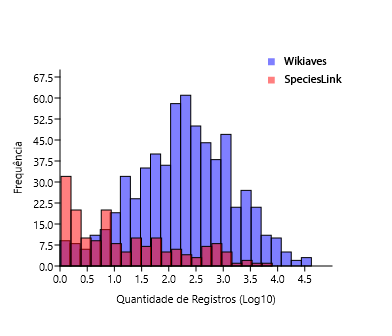
\includegraphics[height = 8cm]{Imagens/H01.png}
\\{\scriptsize Figura 1: Distribuição de municípios em classes segundo o número de registros (Log10), em cada banco de dados: WAV = Wikiaves, SLI = SpeciesLink, WAV2 = WAV com municípios redundantes em SLI. n = número de municípios.  }
\end{figure}

\subsection{Espécies por Município}

\begin{resposta}
As medidas de tendencia central e dispersão para a categoria de espécies por município encontram-se na tabela a seguir: 
\end{resposta}


\begin{figure}[h!]
\centering
{\scriptsize Tabela 3: Estatísticas de tendência central e dispersão para o número de espécies por município em cada banco de dados: WAV = Wikiaves, SLI = SpeciesLink, WAV2 = WAV com municípios redundantes em SLI. Valores de média (m) e desvio-padrão (dp) em Log10 foram retrotransformados (Retro). min-max = valores extremos, q1-q3 = quartis.}
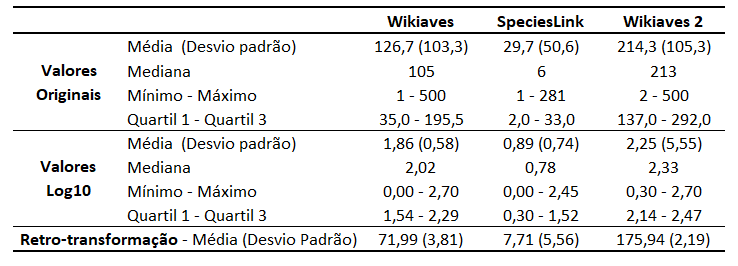
\includegraphics{Imagens/T03.png}
\end{figure}

\begin{resposta}
Há 202 espécies que possuem registro apenas no Wikiaves, enquanto 73 possuem registros apenas no SpeciesLink, os bancos de dados contam com 790 e 661 espécies, respectivamente. A média de espécies por município é, no mínimo, quatro vezes maior para o Wikiaves, é notável que, para tal, o primeiro quartil é maior que o terceiro quartil de seu oposto. Embora isto, a distância entre a média e a mediana é menor nesta base, bem como, o desvio padrão é o dobro em relação à outra, estes valores indicam um padrão mais próximo de uma curva de sino, não obstante, há a necessidade da transformação logarítmica para padronizar os dados do SpeciesLink.

Dentre as 790 espécies que constam no Wikiaves para o estado de São Paulo, 779 possuem registros nos 173 municípios desta análise. O Wikiaves demonstra valores maiores para todos os campos, a distância entre a média e a medina é menor que na seção anterior, os quartis apresentam distância similares entre si, contudo, ainda não são uniformes. É razoável concluir que o Wikiaves apresenta um padrão próximo ao de sino, mesmo para as variáveis originais.

Após transformados, os dados tornam-se mais homogêneos para o SpeciesLink, como esperado, porém ainda não chegam a um padrão. Para o Wikiaves, a mediana torna-se maior que a média, indicando que, de fato, o padrão anterior também se aproxima de uma curva uniforme.

Aplica-se a transformação logarítmica para seguir o procedimento aplicado ao SpeciesLink. Com isto, a mediana para o Wikiaves torna-se maior que a média, a distância entre os quartis é, de certa forma, regular. Contudo, a distância entre o valor mínimo e o primeiro quartil é quase quatro vezes a distância entre o terceiro quartil e o valor máximo.

O SpeciesLink, por certo, não apresenta padrão de sino, por outro lado, o decaimento observado seria maior para as variáveis originais. O Wikiaves está mais próximo deste padrão, distingui-se por, no lugar de decaimento, apresentar uma curva crescente com uma queda intensa ao final.
\end{resposta}



\begin{figure}[h!]
\centering
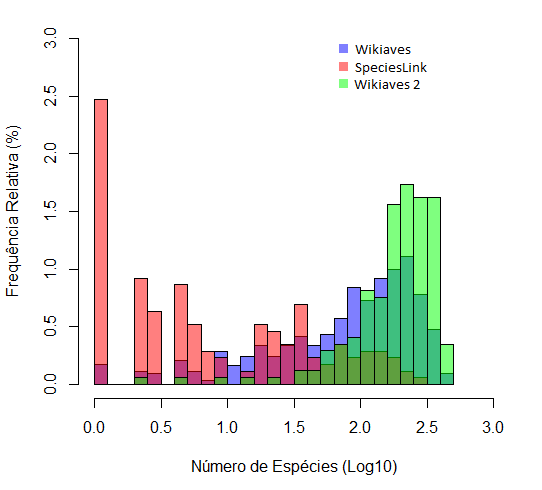
\includegraphics[height = 8cm]{Imagens/H02.png}
\\{\scriptsize Figura 2: Distribuição de municípios em classes segundo o número de espécies (Log10), em cada banco de dados: WAV = Wikiaves, SLI = SpeciesLink, WAV2 = WAV com municípios redundantes em SLI. n = número de municípios. }
\end{figure}


\subsection{Registros por Espécie}

\begin{resposta}
As medidas de tendencia central e dispersão para a categoria de registros por espécie encontram-se na tabela a seguir: 
\end{resposta}

\newpage

\begin{figure}[h!]
\centering
{\scriptsize Tabela 4: Estatísticas de tendência central e dispersão para o número de registros por espécie em cada banco de dados: WAV = Wikiaves, SLI = SpeciesLink, WAV2 = WAV com municípios redundantes em SLI. Valores de média (m) e desvio-padrão (dp) em Log10 foram retrotransformados (Retro). min-max = valores extremos, q1-q3 = quartis.}
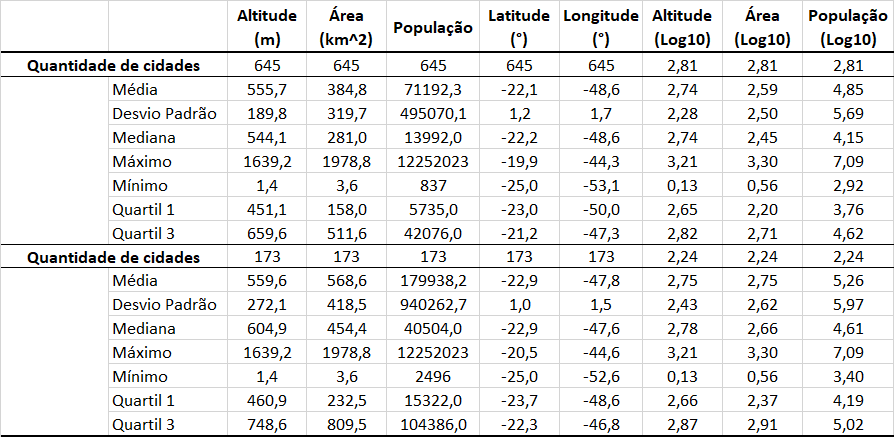
\includegraphics{Imagens/T04.png}
\end{figure}


\begin{resposta}
Para registros por espécie, além da quantidade de registros, a média e a mediana, também, são de uma ordem de grandeza maior para o Wikiaves. Neste, a média é quase o dobro da mediana e o desvio padrão é, inclusive, maior que a média. A distância entre os quartis não é regular para ambos os bancos de dados, no SpeciesLink, a média é maior que o terceiro quartil e o desvio padrão é, no mínimo, quatro vezes a média. Ambos não apresentam um padrão de sino, portanto, aplica-se a transformação logarítmica a fim de uniformizar esses dados. O Wikiaves 2 não se distingue do que foi descrito.

Após a transformação a mediana ultrapassa a média, em ambos, contudo, mais próxima. A distância entre os quartis é mais regular, porém, ainda não é uniforme. No Wikiaves, a distância entre o primeiro quartil e o mínimo é mais em relação à distância entre o terceiro e o máximo. No SpeciesLink, ocorre o oposto, a distância entre o primeiro quartil e o número mínimo é menor que a distância entre o terceiro quartil e o número máximo.
 
\end{resposta}

\begin{figure}[h!]
\centering
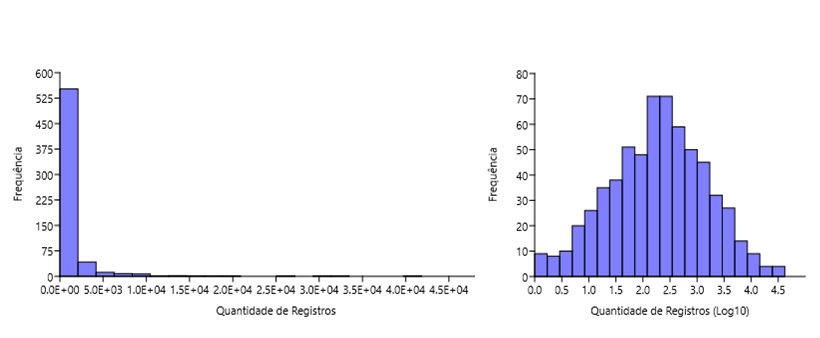
\includegraphics[height = 8cm]{Imagens/H03.png}
\\{\scriptsize Figura 3: Distribuição de espécies em classes segundo o número de registros (Log10), em cada banco de dados: WAV = Wikiaves, SLI = SpeciesLink, WAV2 = WAV com municípios redundantes em SLI. S = número de espécies.}
\end{figure}

\newpage

\section{Fatores Externos}

\begin{resposta}
Em cada seção será apresentada a tabela correspondente aos valores de tendencia central e dispersão para cada varável. Para as analises posteriores serão excluídos os outliers mencionados nesta. Os parâmetros de latitude e longitude são os únicos que não apresentam outliers.
\end{resposta}


\subsection {Altitude}

\begin{figure}[h!]
\centering
{\scriptsize Tabela 5: Estatísticas de tendência central e dispersão para a altitude (m) da sede dos municípios em cada banco de dados: WAV = Wikiaves, SLI = SpeciesLink. n = número de municípios, m = média, dp = desvio-padrão, min-max = valores extremos, q1-q3 = quartis. Foram excluídos dessa análise os municípios com altitude inferior a 250 m e superior a 1200 m.}
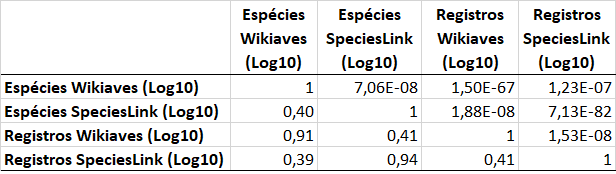
\includegraphics{Imagens/T05.png}
\end{figure}


\begin{resposta}
A Altitude para o Wikiaves apresenta média menor, isto é, as cidades excedentes nesta base, em sua maioria, estão a altitudes mais baixas que a média do SpeciesLink. De fato, o mesmo ocorre para a mediana e os quartis. Foram excluidos os valores maiores e menores que 1200 e 200, respetivamente. Pelos histogramas é possível notar que os bancos de dados apresentam uma quantidade similar de outliers. 
\end{resposta}



\begin{figure}[h!]
\centering
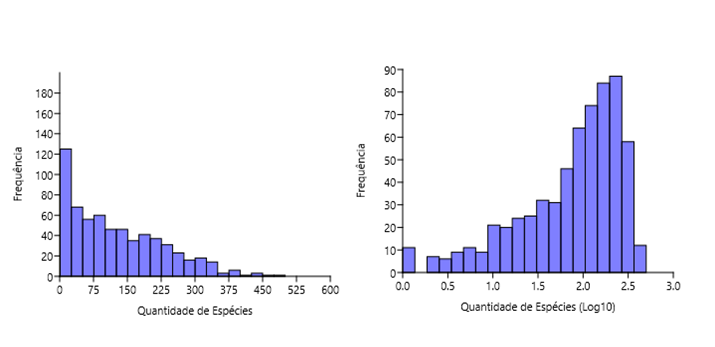
\includegraphics[height = 8cm]{Imagens/H04.png}
\\{\scriptsize Figura 4: Distribuição de municípios em classes segundo a altitude (m) de sua sede em cada banco de dados: WAV = Wikiaves, SLI = SpeciesLink. n = número de municípios. Foram excluídos da análise da Tabela 5 os municípios com altitude inferior a 250 m e superior a 1200 m.}
\end{figure}

\newpage

\subsection{Área}

\begin{figure}[h!]
\centering
{\scriptsize Tabela 6: Estatísticas de tendência central e dispersão para a área (Log10 km2) dos municípios em cada banco de dados: WAV = Wikiaves, SLI = SpeciesLink. n = número de municípios, m = média, dp = desvio-padrão, min-max = valores extremos, q1-q3 = quartis. Foram excluídos dessa análise os municípios com área inferior a X km2.}
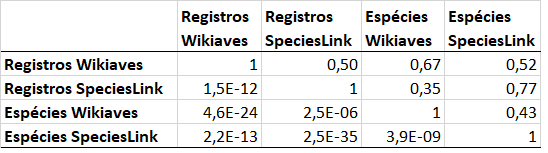
\includegraphics{Imagens/T06.png}
\end{figure}

\begin{resposta}
Observa-se que a média e a mediana ficam próximas, o desvio padrão também é baixo, em relação à análise da seção 1. Foram excluidos os outliers menores que 1,4.
\end{resposta}



\begin{figure}[h!]
\centering
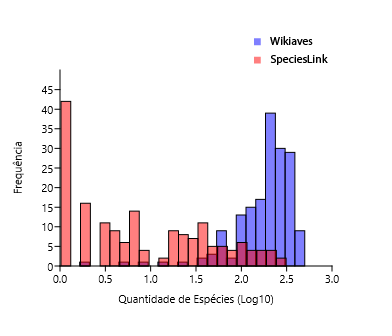
\includegraphics[height = 8cm]{Imagens/H05.png}
\\{\scriptsize Figura 5: Distribuição de municípios em classes segundo a área (Log10 km2) em cada banco de dados: WAV = Wikiaves, SLI = SpeciesLink. n = número de municípios. Foram excluídos da análise da Tabela 6 os municípios com área inferior a X km2.}
\end{figure}

\newpage

\subsection{População}

\begin{figure}[h!]
\centering
{\scriptsize Tabela 7: Estatísticas de tendência central e dispersão para o tamanho da população humana (Log10 indivíduos) dos municípios em cada banco de dados: WAV = Wikiaves, SLI = SpeciesLink. n = número de municípios, m = média, dp = desvio-padrão, min-max = valores extremos, q1-q3 = quartis. Foi excluído dessa análise o município com 12252023 habitantes (São Paulo).}
\\
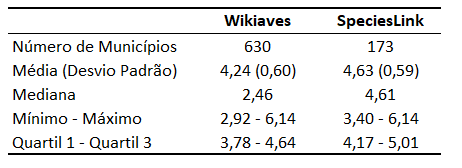
\includegraphics{Imagens/T07.png}
\end{figure}

\begin{resposta}
A média do Wikiaves é menor que a do SpeciesLink, bem como a mediana e os quartis, isto é, o Wikiaves cobre mais cidades menos habitadas. Os dados do SpeciesLink apresentam-se um pouco mais homogêneos, contudo, ambos seguem uma curva de sino quando excluído o mesmo outlier, 7.
\end{resposta}


\begin{figure}[h!]
\centering
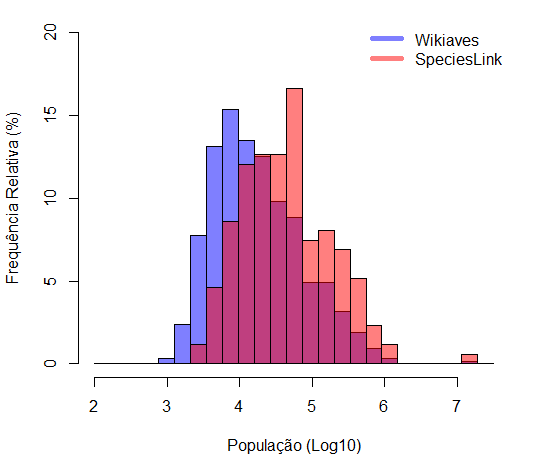
\includegraphics[height = 8cm]{Imagens/H06.png}
\\{\scriptsize Figura 6: Distribuição de municípios em classes segundo o tamanho da população humana (Log10 indivíduos) em cada banco de dados: WAV = Wikiaves, SLI = SpeciesLink. n = número de municípios. Foi excluído da análise da Tabela 7 o município com 12252023 habitantes (São Paulo).}
\end{figure}

\newpage

\subsection{Latitude}

\begin{figure}[h!]
\centering
{\scriptsize Tabela 8: Estatísticas de tendência central e dispersão para a latitude (graus) da sede dos municípios em cada banco de dados: WAV = Wikiaves, SLI = SpeciesLink. n = número de municípios, m = média, dp = desvio-padrão, min-max = valores extremos, q1-q3 = quartis.}
\\
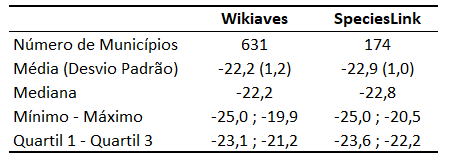
\includegraphics{Imagens/T08.png}
\end{figure}

\begin{resposta}
A princípio as bases de dados possuem uma curva muito parecida, entretanto, para municípios em latitudes mais altas o Wikiaves se sobressai. Os quartis são regulares e o desvio padrão é baixo. 
\end{resposta}

\begin{figure}[h!]
\centering
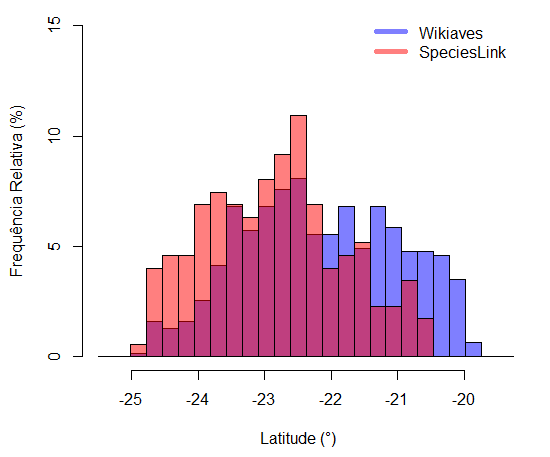
\includegraphics[height = 8cm]{Imagens/H07.png}
\\{\scriptsize Figura 7: Distribuição de municípios em classes a latitude (graus) da sede dos municípios em cada banco de dados: WAV = Wikiaves, SLI = SpeciesLink. n = número de municípios.}
\end{figure}

\newpage

\subsection{Longitude}


\begin{figure}[h!]
\centering
{\scriptsize Tabela 9: Estatísticas de tendência central e dispersão para a longitude (graus) da sede dos municípios em cada banco de dados: WAV = Wikiaves, SLI = SpeciesLink. n = número de municípios, m = média, dp = desvio-padrão, min-max = valores extremos, q1-q3 = quartis.}
\\
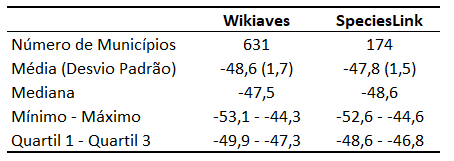
\includegraphics{Imagens/T09.png}
\end{figure}

\begin{resposta}
O Wikiaves possui mais cidades em longitudes mais baixas, além disto, sua média é igual à mediana e o desvio padrão é baixo, com intervalo quase regular entre os quartis. Para o SpeciesLink, o padrão de baixo desvio padrão se mantém, mas, a regularidade da distância dos quartis é menor.
\end{resposta}


\begin{figure}[h!]
\centering
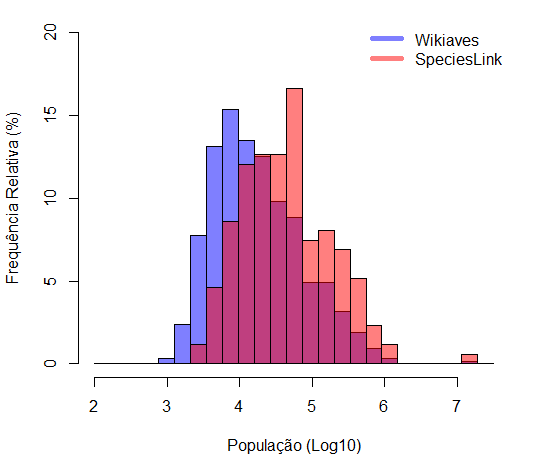
\includegraphics[height = 8cm]{Imagens/H06.png}
\\{\scriptsize Figura 8: Distribuição de municípios em classes a longitude (graus) da sede dos municípios em cada banco de dados: WAV = Wikiaves, SLI = SpeciesLink. n = número de municípios.}
\end{figure}

\newpage

\section{Análise Bivariada}

\hrulefill

\hrulefill



\subsection{Registros}

\begin{resposta}
Os valores de correlação, valor-p e número de municípios encontram-se na tabela a seguir:
\end{resposta}


\begin{figure}[h!]
\centering
{\scriptsize Tabela 10. Correlação linear entre o número de registros (Log10) por município em cada banco de dados e variáveis explanatórias. WAV = Wikiaves, SLI = SpeciesLink, WAV2 = WAV com municípios redundantes em SLI. Número de municípios (n), coeficiente de correlação de Pearson (r) para cada pareamento, com outliers bivariados excluídos. Valores significantes $(p < 0.05)$ em negrito. }
\\
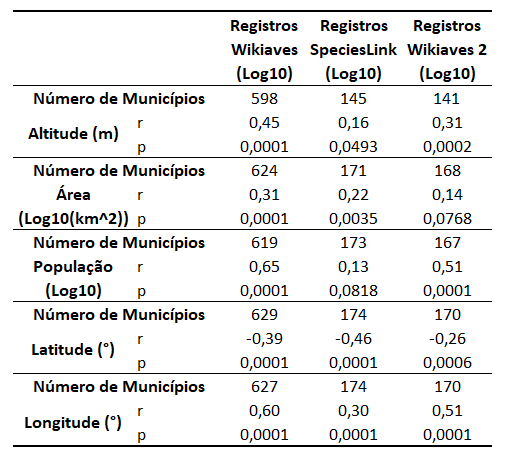
\includegraphics{Imagens/T10.png}
\end{figure}

 

\subsubsection{Altitude}

\begin{figure}[h!]
\centering
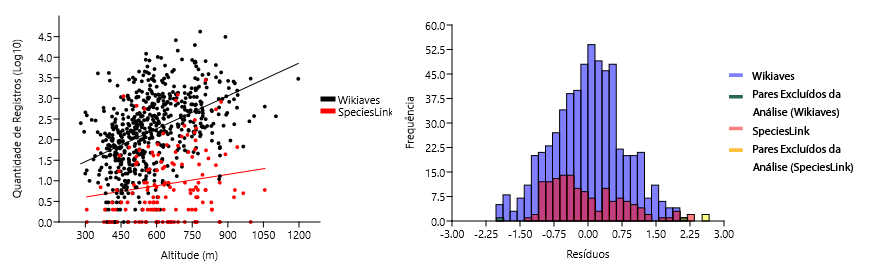
\includegraphics[width = 15cm]{Imagens/G01.png}
\\{\scriptsize Figura 9. Relação linear entre o número de registros (Log10) em cada banco de dados e a altitude (m) da sede dos municípios (esquerda) e respectiva distribuição de resíduos (direita, em unidades de desvio-padrão, em unidades de desvio-padrão). Outliers bivariados foram excluídos. }
\end{figure}
\newpage

\begin{resposta}
Para o estado de São Paulo, embora hajam valores baixos de $p$ para o Wikiaves, o espaço amostral é de 598 municípios, portanto, espera-se que estes valores sejam pequenos. Para o SpeciesLink, a medida de $p$ que é maior que $0,01$, está próxima a este valor. O gráfico abaixo servirá de indicativo para determinar se a evidência coletada é o suficiente para a rejeição da hipótese nula.

De fato, a quantidade de registros no Wikiaves aumenta conforme o aumento de altitude. Contudo, não é um aumento evidente, há muitos pares ordenados distantes da reta, isto é, a reta de regressão neste caso não é uma boa aproximação para esta curva. Para o SpeciesLink, os gráficos explicitam que o valor de $p < 0,05$ e próximo a $0,01$ não é o suficiente para a rejeição da hipótese nula, na verdade, os dados mostram-se distantes da reta e sem padrão definido.

Quanto aos municípios registrados em ambos os bancos de dados, percebe-se, no Wikiaves, um aumento relevante do valor de $p$, que pode ser explicado pela diminuição da quantidade de cidades. 
\end{resposta}



\subsubsection{Área}


\begin{figure}[h!]
\centering
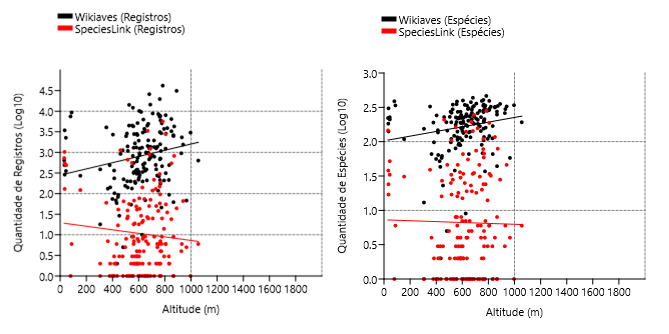
\includegraphics[width = 15cm]{Imagens/G02.png}
\\{\scriptsize Figura 10. Relação linear entre o número de registros (Log10) em cada banco de dados e a área (Log10 km2) dos municípios (esquerda) e respectiva distribuição de resíduos (direita, em unidades de desvio-padrão). Outliers bivariados foram excluídos.}
\end{figure}

\begin{resposta}
 Os valores de correlação linear para os municípios registrados no Wikiaves ou no SpeciesLink são de $0,31$ e $0,22$, respectivamente. Devido aos baixos valores de $p$ é possível que haja uma correlação não linear entre o que analisando, para confirmar ou contestar isto, atente-se ao gráfico: 
 
 É relevante que não há outliers bivariados. Além disto, há, de fato, um aumento linear, apesar disto, os pares ordenados encontram-se dispersos da reta de regressão, o que explica os baixos valores de correlação.

Ao diminuir a quantidade de cidades no Wikiaves, os valores de $p$ aumentam, torna-se maior que $0,01$, seguidos de valores baixos de $r$ em ambos. 

De fato, é possível afirmar que este parâmetro não possui grande influência sobre a quantidade de registros nas duas bases.
\end{resposta}



\subsubsection{População}

\begin{figure}[h!]
\centering
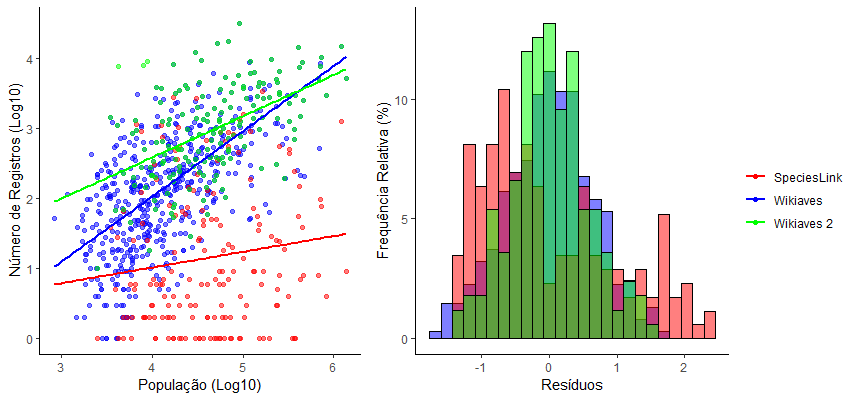
\includegraphics[width = 15cm]{Imagens/G03.png}
\\{\scriptsize Figura 11. Relação linear entre o número de registros (Log10) em cada banco de dados e o tamanho da população humana (Log10 indivíduos) dos municípios (esquerda) e respectiva distribuição de resíduos (direita, em unidades de desvio-padrão). Outliers bivariados foram excluídos.}
\end{figure}

\begin{resposta}
 O valor de correlação para os 619 municípios analisados para o Wikiaves é o maior obtido até então: $0,65$, um forte indicativo que há correlação linear nesta base. Em contrapartida, o SpeciesLink apresenta $p = 0,08$, que é um valor que exige cautela, como a correlação nesta base é de $0,13$ é possível assumir que não há correlação linear. Os gráficos a seguir confirmam isto.
 
\end{resposta}

\subsubsection{Latitude}

\begin{figure}[h!]
\centering
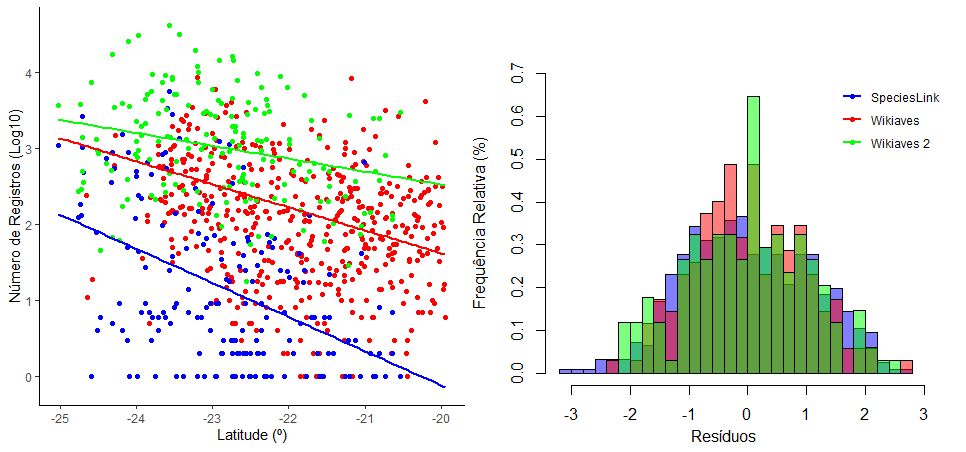
\includegraphics[width = 15cm]{Imagens/G04.png}
\\{\scriptsize Figura 12. Relação linear entre o número de registros (Log10) em cada banco de dados e a latitude (graus) da sede dos municípios (esquerda) e respectiva distribuição de resíduos (direita, em unidades de desvio-padrão). Outliers bivariados foram excluídos.}
\end{figure}

\newpage

\begin{resposta}
 Os valores de $p$ e $r$, aparentam ser o suficiente para constatar que há um decaimento na quantidade de registros conforme aumento de altitude. 
 
 Os resíduos são regulares ao passo que estão dispersos da reta de regressão, há correlação linear, porém é baixa. Ao retirar as cidades excedentes os valores aumentam (no caso, o relacionamento é menor) no Wikiaves.
\end{resposta}

\subsubsection{Longitude}

\begin{figure}[h!]
\centering
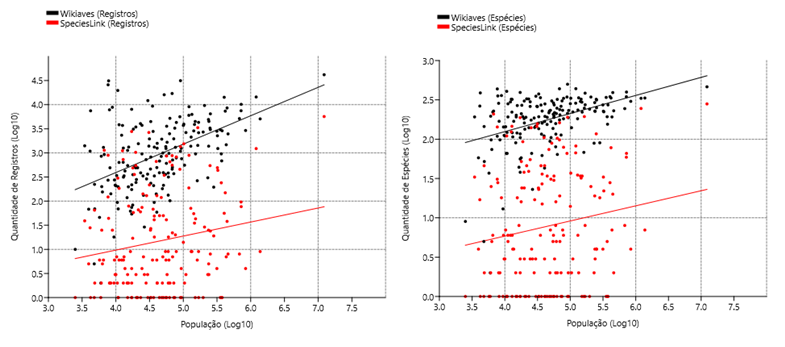
\includegraphics[width = 15cm]{Imagens/G05.png}
\\{\scriptsize Figura 13. Relação linear entre o número de registros (Log10) em cada banco de dados e a longitude (graus) da sede dos municípios (esquerda) e respectiva distribuição de resíduos (direita, em unidades de desvio-padrão). Outliers bivariados foram excluídos.}
\end{figure}

 \begin{resposta}
O aumento linear é claro no Wikiaves e, embora não seja tão evidente assim, há um aumento no SpeciesLink, também.

Os resíduos regulares, bem como, o aumento no gráfico indicam que há relação.
\end{resposta}


\subsection{Espécies}

\begin{resposta}
Os valores de correlação, valor-p e número de municípios encontram-se na tabela a seguir:
\end{resposta}

\newpage

\begin{figure}[h!]
\centering
{\scriptsize Tabela 11: Correlação linear entre o número de espécies (Log10) por município em cada banco de dados e variáveis explanatórias. WAV = Wikiaves, SLI = SpeciesLink, WAV2 = WAV com municípios redundantes em SLI. Número de municípios (n), coeficiente de correlação de Pearson (r) para cada pareamento, com outliers bivariados excluídos. Valores significantes $(p < 0.05)$ em negrito.}
\\
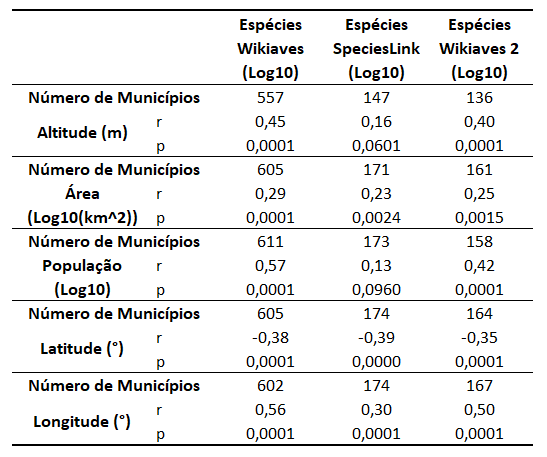
\includegraphics{Imagens/T11.png}
\end{figure}

\subsubsection{Altitude}


 

\begin{figure}[h!]
\centering
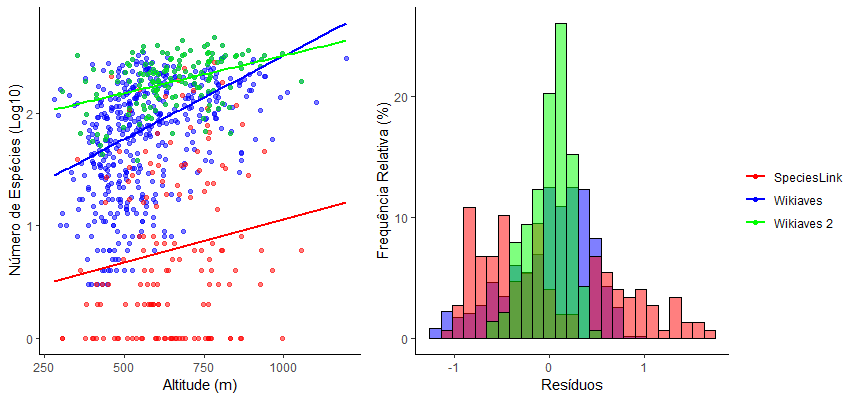
\includegraphics[width = 15cm]{Imagens/G06.png}
\\{\scriptsize Figura 14: Relação linear entre o número de espécies (Log10) em cada banco de dados e a altitude (m) da sede dos municípios (esquerda) e respectiva distribuição de resíduos (direita, em unidades de desvio-padrão). Outliers bivariados foram excluídos.}
\end{figure}


\begin{resposta}
Os valores de $p$ para a quantidade de espécies são, ainda, maiores que os que dizem respeito aos registros, neste cenário, é possível assumir que não há relação entre a altitude e os dados do SpeciesLink ($p > 0,05$). No caso da outra base, os valores de $p$ são baixos o suficiente para que haja relação. O gráfico abaixo explicita o comportamento. Novamente, os dados estão dispersos da linha de tendência no Wikiaves. No SpeciesLink, de fato, não há correlação linear.

Ao admitir apenas os 173 municípios registrados por ambas as bases, o valor de $p$ para o Wikiaves não sofre uma mudança tão drástica quanto para os registros, na verdade, este valor continua abaixo de $0,01$. Note, no gráfico abaixo, que os valores não estão dispersos da linha de tendência, portanto, pode assumir que há uma relação.
\end{resposta}

\subsubsection{Área}



\begin{figure}[h!]
\centering
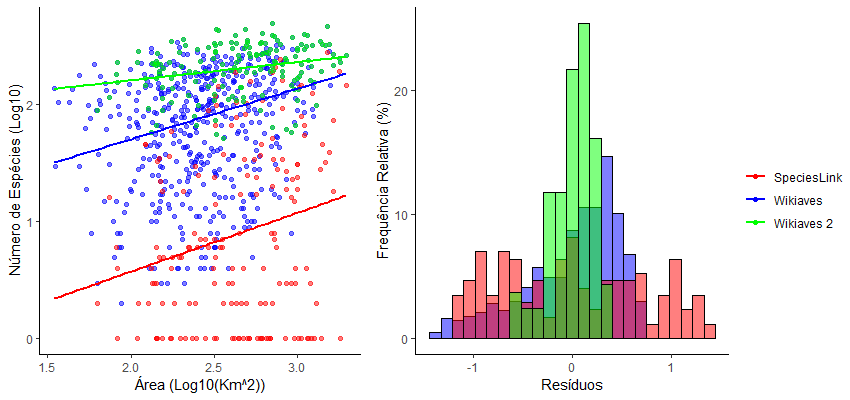
\includegraphics[width = 15cm]{Imagens/G07.png}
\\{\scriptsize Figura 15: Relação linear entre o número de espécies (Log10) em cada banco de dados e a área (Log10 km2) dos municípios (esquerda) e respectiva distribuição de resíduos (direita, em unidades de desvio-padrão). Outliers bivariados foram excluídos.}
\end{figure}

 \begin{resposta}
Quanto a quantidade de espécies os valores de $r$ diminuem no Wikiaves e aumentam no SpeciesLink, entretanto, não o suficiente para concluir que há ou não correlação linear entre as variáveis.

Tanto pelo gráfico quanto pelo modo com o qual os resíduos estão distribuídos identifica-se que não há correlação linear entre os dados. A situação não se altera ao se retirar os municípios excedentes. No geral, o tamanho de um município não possui grande influência em relação as variáveis resposta.
\end{resposta}

\subsubsection{População}

 \newpage

\begin{figure}[h!]
\centering
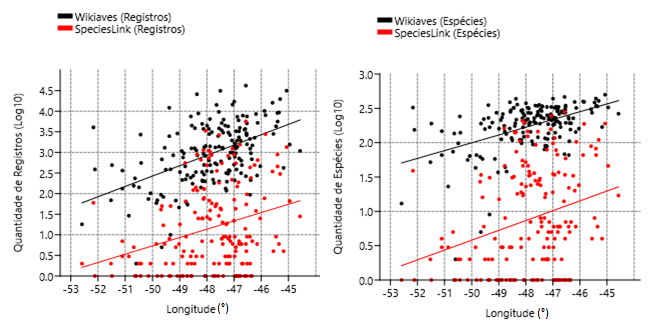
\includegraphics[width = 15cm]{Imagens/G08.png}
\\{\scriptsize Figura 16: Relação linear entre o número de espécies (Log10) em cada banco de dados e o tamanho da população humana (Log10 indivíduos) dos municípios (esquerda) e respectiva distribuição de resíduos (direita, em unidades de desvio-padrão). Outliers bivariados foram excluídos.}
\end{figure}

\begin{resposta}
De forma semelhante aos registros, a quantidade de espécies parece seguir o mesmo padrão. O valor de correlação é menor, percebe-se pelo gráfico que há relação para o Wikiaves. De fato, há um crescimento no Wikiaves, vez que, o SpeciesLink não segue padrão algum. Ao retirar os municípios excedentes o coeficiente angular da reta do Wikiaves aproxima-se de 0, ainda, é possível observar a relação.

Conclui-se que, este parâmetro influencia o Wikiaves, apenas. Ou seja, as bases de dados divergem quanto ao comportamento analisado nesta seção.
\end{resposta}

\subsubsection{Latitude}

 

\begin{figure}[h!]
\centering
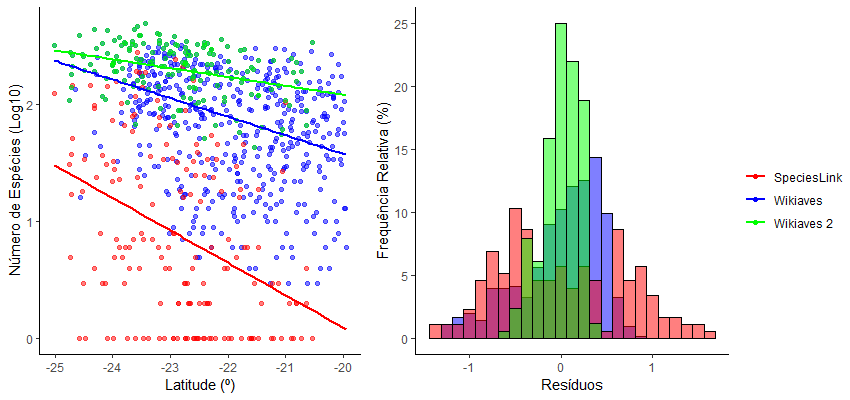
\includegraphics[width = 15cm]{Imagens/G09.png}
\\{\scriptsize Figura 17: Relação linear entre o número de espécies (Log10) em cada banco de dados e a latitude (graus) da sede dos municípios (esquerda) e respectiva distribuição de resíduos (direita, em unidades de desvio-padrão). Outliers bivariados foram excluídos.}
\end{figure}

\begin{resposta}
Para a quantidade de espécies os bancos de dados apresentam valores próximos de $r$. Note o comportamento nos gráficos:

O valor dos resíduos no Wikiaves aumentam conforme aumento da altitude e, no SpeciesLink, ocorre o oposto. No geral, assume-se uma correlação fraca entre este fator e a quantidade de espécies. De fato, o mesmo vale para quando se retira os municípios com registro em apenas uma das bases.
\end{resposta}

\subsubsection{Longitude}

\begin{figure}[h!]
\centering
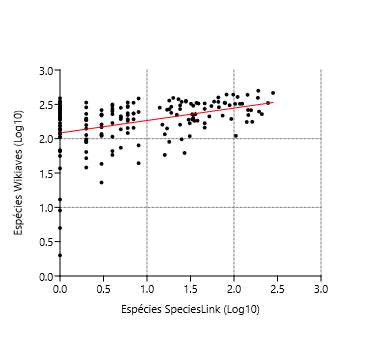
\includegraphics[width = 15cm]{Imagens/G10.png}
\\{\scriptsize Figura 18: Relação linear entre o número de espécies (Log10) em cada banco de dados e a longitude (graus) da sede dos municípios (esquerda) e respectiva distribuição de resíduos (direita, em unidades de desvio-padrão). Outliers bivariados foram excluídos.}
\end{figure}

 \begin{resposta}
Novamente, os pares ordenados estão dispersos da linha de tendência, contudo, os quartis regulares e o crescimento são indícios de que há relação. Isso se mantém ao retirar os municípios com registro em apenas uma das bases.
\end{resposta}


\section{Metodologia}

\subsection{Materiais e Métodos}

No período de janeiro a fevereiro de 2020, foram coletados os registros provenientes de cientistas-cidadãos no portal Wikiaves (WikiAves, 2020) e aqueles provenientes de cientistas nas coleções disponíveis na rede SpeciesLink (2020).

Para responder às questões supracitadas, foram utilizadas as seguintes variáveis oriundas dos dois bancos de dados: o número de registros de cada espécie por município, o número de espécies registradas por município e suas versões log-transformadas (base 10). Foram empregadas, também, variáveis explanatórias, sendo elas: a altitude da sede, logaritmo na base 10 área, logaritmo na base 10 da quantidade de habitantes, latitude e longitude referentes a cada município. Todas as informações quanto as variáveis explanatórias foram obtidas no sítio do IBGE (2020). Os biomas predominantes em cada município serão determinados de acordo com o sítio MapBiomas (2020).

 As abordagens discriminadas serão conduzidas com os programas R \cite{CoreTeam2017}.

\subsection{Etapas da pesquisa}

\color{blue}\textit{Aqui começam a surgir algumas dúvidas, não mantive a folha de considerações para não atrapalhar a estrutura do texto, vou colocar as considerações ao longo do texto, porém, em itálico e azul.\\ A primeira delas é que eu não sei se posso adicionar subsubseções ao modelo da ufabc, acredito que não, de todo modo o fiz neste primeiro momento por um questão de organização, apenas.}\color{black}

A principio, para equiparação dos bancos de dados, as espécies foram denominadas em acordo com a lista das aves do Brasil do Comitê Brasileiro de Registros Ornitológicos \cite{De2015}.

\subsubsection{Análise Univariada}

Para medir a normalidade dos dados coletados foi empregada uma análise exploratória de dados \cite{NicholasJ.Gotelli;AaronM.Ellison2010,Field2012, Borcard2011}. Foram calculados, portanto, as estatísticas de posição (média, mediana e quartis), dispersão (desvio padrão), inclinação e curtose.  \color{blue}\textit{(Ok, mais um grande parenteses aqui, eu não falei de inclinação e curtose até agora porque (me perdoe) eu tinha esquecido desses valores, eles estavam na planilha que eu estava usando quando fiz as análises no past, ela foi arquivada e eles ficaram perdidos. Para escrever o trabalho de maneira mais formal, tive que reler algumas referências e lembrei que esses valores podem ser importantes (o valor de curtose no WAV2 para a quantidade de espécies é de 11.50854, o que eu acho que é um valor alto), se eles forem importantes, posso apresenta-los nas tabelas.)}\color{black}. Foram removidos os valores discrepantes relativos às variáveis explanatórias \cite{VALENTIN2000,Field2012} e aplicada a transformação logarítmica para todas as variavéis exceto: altitude, latitude e longitude \cite{NicholasJ.Gotelli;AaronM.Ellison2010,Field2012,Borcard2011}. \color{blue}\textit{(Anteriormente eu falei que foram utilizadas as versões log-transformadas. Acredito que isto seja um pleonasmo, mas não sei se esta informação deve aparecer aqui ou lá.)}\color{black}. Os dados foram impressos como gráficos de linhas. \color{blue}\textit{(Eu gostei da apresentação dos gráficos de linha, mas, não me lembro de nenhum livro que justifique isto, então deixei sem citação.)}\color{black}



\subsubsection{Análise Bivariada}

A partir dos dados reformatados após a análise anterior, foi estabelecido um exame quanto a regressão linear dos parâmetros apresentados \cite{NicholasJ.Gotelli;AaronM.Ellison2010}. Foram medidos os valores de $r^2$, $p$, a inclinação da reta e o intercepto para como cada variável preditora (quantidade de registros e espécies próprias de cada banco de dados) modifica-se conforme alteração nas variáveis explanatórias e como as variáveis preditoras modificam-se entre si, isto é, variação da quantidade de registros de um banco de dados (analogamente, espécies) conforme alteração da quantidade de registros do outro. Os pares-ordenados com resíduos discrepantes foram excluídos \cite{Field2012}.

Por fins de encontrar a variação na quantidade de registros conforme a quantidade de espécies adotou-se um modelo de regressão não linear \cite{NicholasJ.Gotelli;AaronM.Ellison2010}, a partir deste, foram calculados os valores de $r^2$, $p$, inclinação da reta e intercepto.

Para uma análise visual dos dados foram aplicados gráficos de dispersão ao modelo de regressão \cite{NicholasJ.Gotelli;AaronM.Ellison2010} e gráficos de linha para os resíduos.

\subsubsection{Distribuição Geográfica}

Foram construídos mapas temáticas que apresentam as de acordo com a distribuição geográfica de cada uma \cite{Borcard2011}. \color{blue}\textit{(O Borcard traz essa questão de mostrar as variáveis conforme a localização de cada registro, porém, não do mesmo modo que fizemos, acredito que entre como citação aqui (?).)}\color{black}

\subsubsection{Análise de Covariância}

Comparações entre curvas serão feitas por análise de covariância \cite{NicholasJ.Gotelli;AaronM.Ellison2010,Borcard2011, Field2012}.

\subsubsection{Análise de Classificação}

Para a realização de uma análise multivariada, foram desenvolvidas matrizes de distância, valendo-se do valor de similaridade de Jaccard \cite{VALENTIN2000,greenacre2014multivariate}, fundamentados nestas matrizes foram construídos dendogramas hierárquicos para determinar grupos de cidades similares conforme a composição de espécies \cite{VALENTIN2000,greenacre2014multivariate,Borcard2011}.

A posteriori, serão elaborados mapas coloridos conforme os grupos descritos acima e será empregado o teste de mantel para comparar as matrizes de distância \cite{Borcard2011,VALENTIN2000}.


\section{Resultados e discussão dos resultados}

\color{blue}\textit{Acredito que deva haver um modo bem melhor para organizar tudo isso, eu posso reunir gráficos em blocos? Assim como foi feito para os mapas de registros e espécies (até porque há 14 páginas só de imagens).}\color{black}

\subsection{Análise Univariada}

\begin{figure}[h!]
\centering
{\scriptsize Tabela 1: Número de municípios amostrados, registros e espécies nos bancos de dados: WAV = Wikiaves, SLI = SpeciesLink, WAV2 = WAV com municípios redundantes em SLI.}
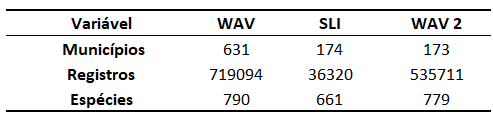
\includegraphics{Tabelas/1.png}
\label{t01}
\end{figure}

\begin{itemize}
    \item Registros por Município

\begin{figure}[h!]
\centering
{\scriptsize Tabela 2: Estatísticas de tendência central e dispersão para o número de registros por município em cada banco de dados: WAV = Wikiaves, SLI = SpeciesLink, WAV2 = WAV com municípios redundantes em SLI. Valores de média (m) e desvio-padrão (dp) em Log10 foram retrotransformados (Retro). min-max = valores extremos, q1-q3 = quartis.}
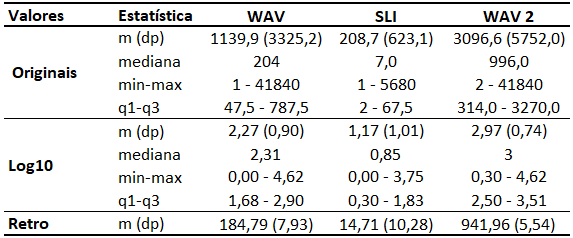
\includegraphics[height = 4cm]{Tabelas/2.png}
\label{t02}
\end{figure}

\begin{figure}[h!]
\centering
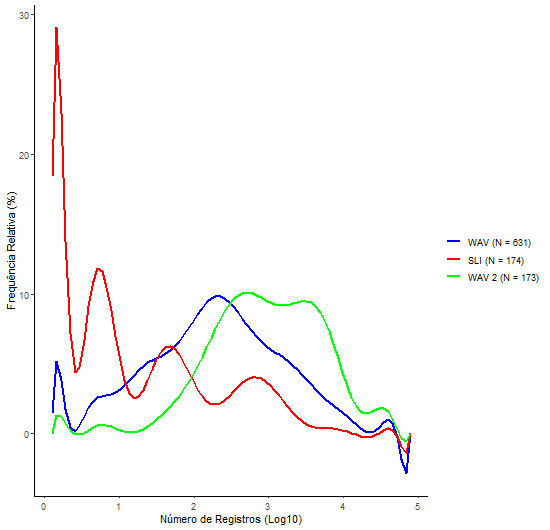
\includegraphics[height = 6cm]{Imagens/113.png}
\\{\scriptsize Figura 1: Distribuição de municípios em classes segundo o número de registros (Log10), em cada banco de dados: WAV = Wikiaves, SLI = SpeciesLink, WAV2 = WAV com municípios redundantes em SLI. n = número de municípios.  }
\label{fig01}
\end{figure}



\item Espécies por Município

\begin{figure}[h!]
\centering
{\scriptsize Tabela 3: Estatísticas de tendência central e dispersão para o número de espécies por município em cada banco de dados: WAV = Wikiaves, SLI = SpeciesLink, WAV2 = WAV com municípios redundantes em SLI. Valores de média (m) e desvio-padrão (dp) em Log10 foram retrotransformados (Retro). min-max = valores extremos, q1-q3 = quartis.}
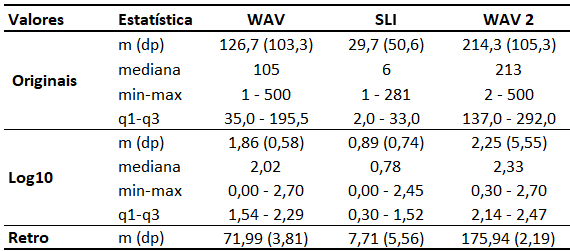
\includegraphics[height = 4cm]{Tabelas/3.png}
\label{t03}
\end{figure}


\begin{figure}[h!]
\centering
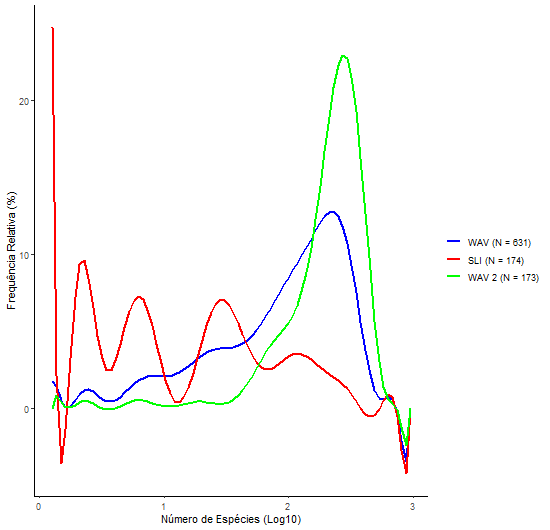
\includegraphics[height = 6cm]{Imagens/123.png}
\\{\scriptsize Figura 2: Distribuição de municípios em classes segundo o número de espécies (Log10), em cada banco de dados: WAV = Wikiaves, SLI = SpeciesLink, WAV2 = WAV com municípios redundantes em SLI. n = número de municípios. }
\label{fig02}
\end{figure}

\newpage

\item Registros por Espécie

\begin{figure}[h!]
\centering
{\scriptsize Tabela 4: Estatísticas de tendência central e dispersão para o número de registros por espécie em cada banco de dados: WAV = Wikiaves, SLI = SpeciesLink, WAV2 = WAV com municípios redundantes em SLI. Valores de média (m) e desvio-padrão (dp) em Log10 foram retrotransformados (Retro). min-max = valores extremos, q1-q3 = quartis.}
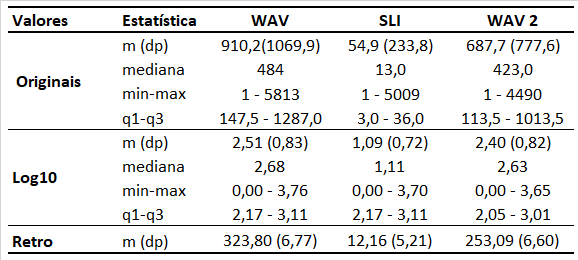
\includegraphics[height = 4cm]{Tabelas/4.png}
\label{t04}
\end{figure}

\begin{figure}[h!]
\centering
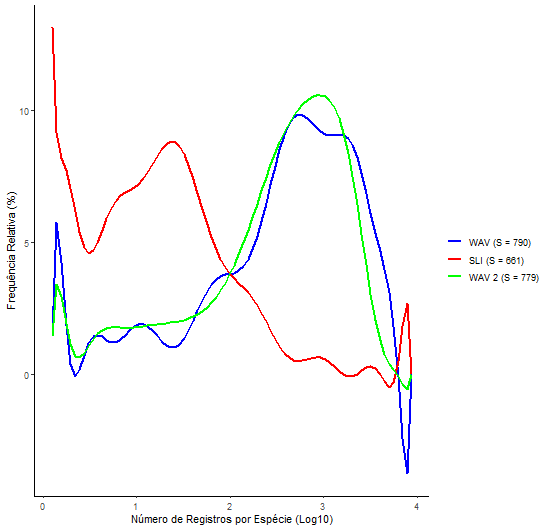
\includegraphics[height = 6cm]{Imagens/133.png}
\\{\scriptsize Figura 3: Distribuição de espécies em classes segundo o número de registros (Log10), em cada banco de dados: WAV = Wikiaves, SLI = SpeciesLink, WAV2 = WAV com municípios redundantes em SLI. S = número de espécies.}
\label{fig03}
\end{figure}

\newpage

\item Altitude

\begin{figure}[h!]
\centering
{\scriptsize Tabela 5: Estatísticas de tendência central e dispersão para a altitude (m) da sede dos municípios em cada banco de dados: WAV = Wikiaves, SLI = SpeciesLink. n = número de municípios, m = média, dp = desvio-padrão, min-max = valores extremos, q1-q3 = quartis. Foram excluídos dessa análise os municípios com altitude inferior a 250 m e superior a 1200 m.}
\\
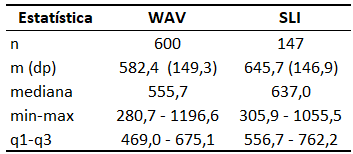
\includegraphics[height = 3cm]{Tabelas/5.png}
\label{t05}
\end{figure}

\begin{figure}[h!]
\centering
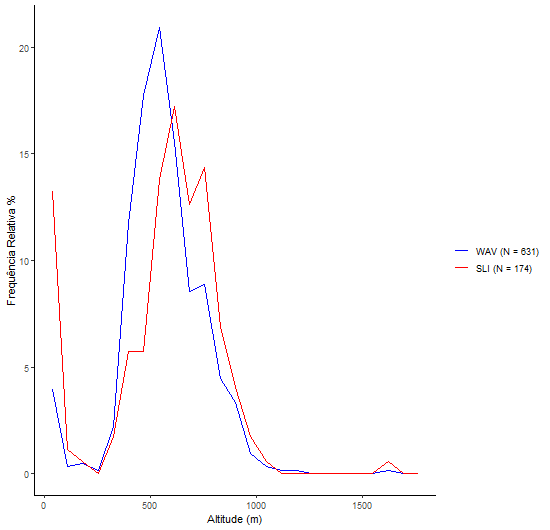
\includegraphics[height = 6cm]{Imagens/213.png}
\\{\scriptsize Figura 4: Distribuição de municípios em classes segundo a altitude (m) de sua sede em cada banco de dados: WAV = Wikiaves, SLI = SpeciesLink. n = número de municípios. Foram excluídos da análise da Tabela 5 os municípios com altitude inferior a 250 m e superior a 1200 m.}
\end{figure}

\item Área

\begin{figure}[h!]
\centering
{\scriptsize Tabela 6: Estatísticas de tendência central e dispersão para a área (Log10 km2) dos municípios em cada banco de dados: WAV = Wikiaves, SLI = SpeciesLink. n = número de municípios, m = média, dp = desvio-padrão, min-max = valores extremos, q1-q3 = quartis. Foram excluídos dessa análise os municípios com área inferior a 20 km2 no WAV e 40km2 no SLI.}
\\
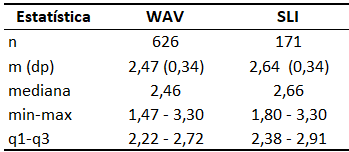
\includegraphics[height = 3cm]{Tabelas/6.png}
\end{figure}

\newpage

\begin{figure}[h!]
\centering
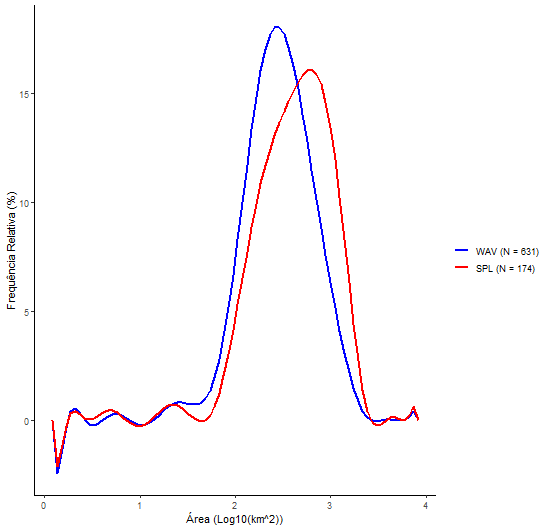
\includegraphics[height = 6cm]{Imagens/223.png}
\\{\scriptsize Figura 5: Distribuição de municípios em classes segundo a área (Log10 km2) em cada banco de dados: WAV = Wikiaves, SLI = SpeciesLink. n = número de municípios. Foram excluídos da análise da Tabela 6 os municípios com área inferior a 20 km2 no WAV e 40km2 no SLI.}
\end{figure}


\item População

\begin{figure}[h!]
\centering
{\scriptsize Tabela 7: Estatísticas de tendência central e dispersão para o tamanho da população humana (Log10 indivíduos) dos municípios em cada banco de dados: WAV = Wikiaves, SLI = SpeciesLink. n = número de municípios, m = média, dp = desvio-padrão, min-max = valores extremos, q1-q3 = quartis. Foi excluído dessa análise o município com 12252023 habitantes (São Paulo).}
\\
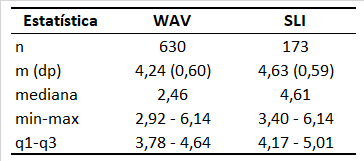
\includegraphics[height = 3cm]{Tabelas/7.png}
\end{figure}



\begin{figure}[h!]
\centering
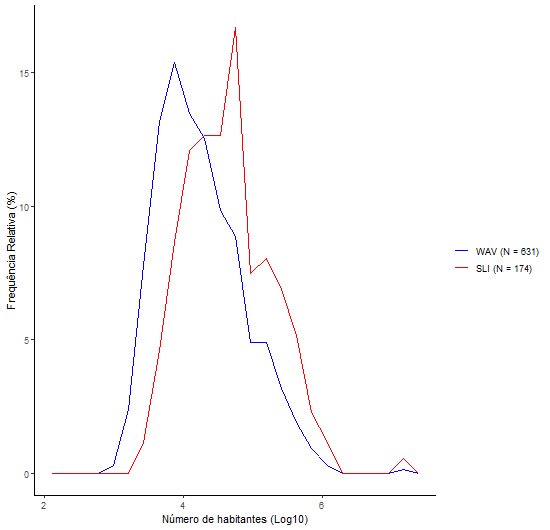
\includegraphics[height = 6cm]{Imagens/233.png}
\\{\scriptsize Figura 6: Distribuição de municípios em classes segundo o tamanho da população humana (Log10 indivíduos) em cada banco de dados: WAV = Wikiaves, SLI = SpeciesLink. n = número de municípios. Foi excluído da análise da Tabela 7 o município com 12252023 habitantes (São Paulo).}
\end{figure}

\newpage

\item Latitude

\begin{figure}[h!]
\centering
{\scriptsize Tabela 8: Estatísticas de tendência central e dispersão para a latitude (graus) da sede dos municípios em cada banco de dados: WAV = Wikiaves, SLI = SpeciesLink. n = número de municípios, m = média, dp = desvio-padrão, min-max = valores extremos, q1-q3 = quartis.}
\\
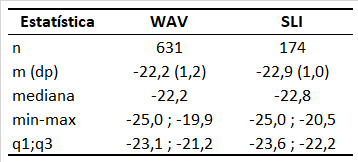
\includegraphics[height = 3cm]{Tabelas/8.png}
\end{figure}



\begin{figure}[h!]
\centering
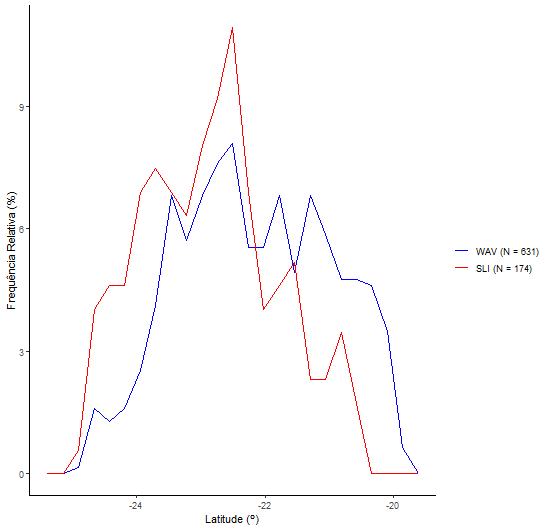
\includegraphics[height = 6cm]{Imagens/243.png}
\\{\scriptsize Figura 7: Distribuição de municípios em classes a latitude (graus) da sede dos municípios em cada banco de dados: WAV = Wikiaves, SLI = SpeciesLink. n = número de municípios.}
\end{figure}

\item Longitude


\begin{figure}[h!]
\centering
{\scriptsize Tabela 9: Estatísticas de tendência central e dispersão para a longitude (graus) da sede dos municípios em cada banco de dados: WAV = Wikiaves, SLI = SpeciesLink. n = número de municípios, m = média, dp = desvio-padrão, min-max = valores extremos, q1-q3 = quartis.}
\\
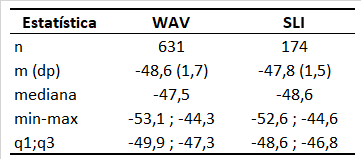
\includegraphics[height = 3cm]{Tabelas/9.png}
\end{figure}


\begin{figure}[h!]
\centering
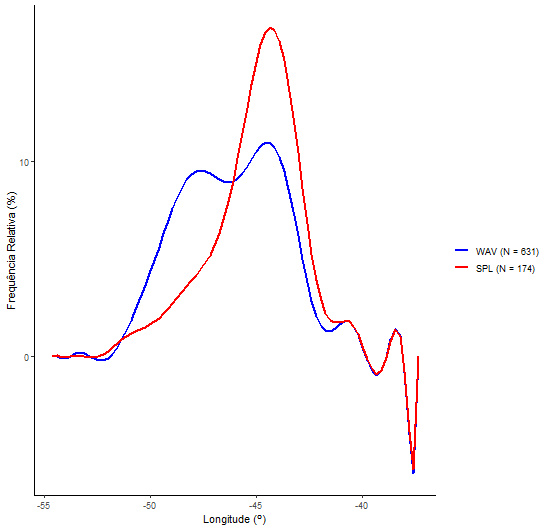
\includegraphics[height = 6cm]{Imagens/253.png}
\\{\scriptsize Figura 8: Distribuição de municípios em classes a longitude (graus) da sede dos municípios em cada banco de dados: WAV = Wikiaves, SLI = SpeciesLink. n = número de municípios.}
\end{figure}

\end{itemize}

\newpage

\subsection{Análise Bivariada}

\begin{itemize}

\item Registros

\begin{figure}[h!]
\centering
{\scriptsize Tabela 10. Correlação linear entre o número de registros (Log10) por município em cada banco de dados e variáveis explanatórias. WAV = Wikiaves, SLI = SpeciesLink, WAV2 = WAV com municípios redundantes em SLI. Número de municípios (n), coeficiente de correlação de Pearson (r) para cada pareamento, com outliers bivariados excluídos. Valores significantes $(p < 0.05)$ em negrito. }
\\
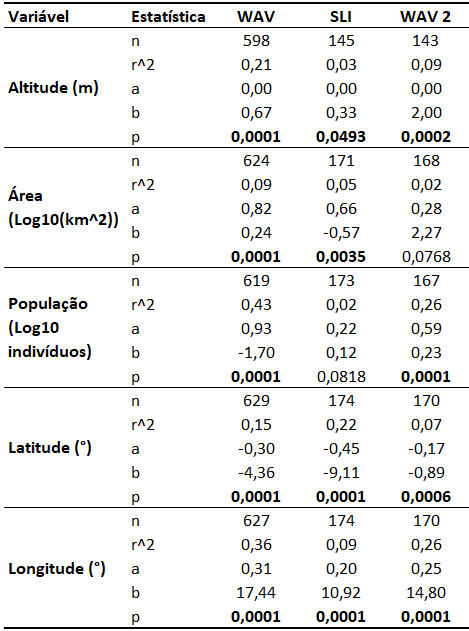
\includegraphics[height = 11cm]{Tabelas/10.png}
\end{figure}

\newpage

\begin{itemize}

\item Altitude

\begin{figure}[h!]
\centering
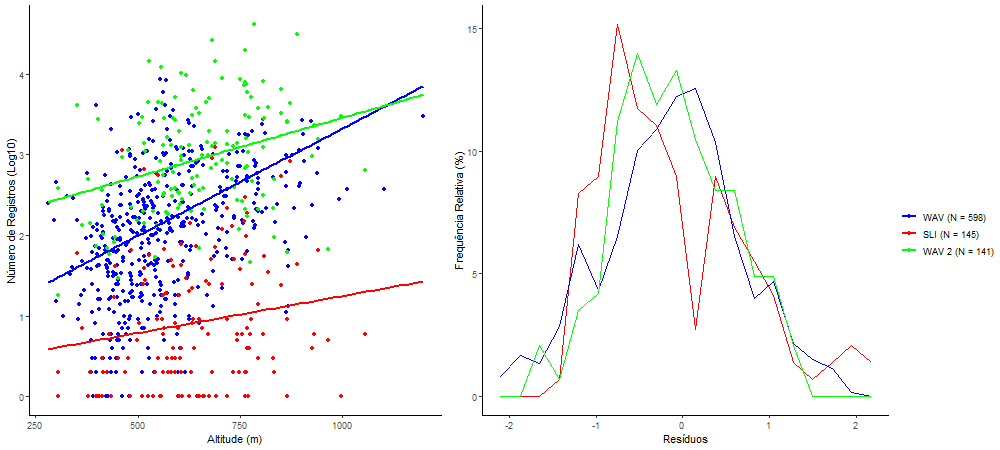
\includegraphics[width = 15cm]{Imagens/31113.png}
\\{\scriptsize Figura 9. Relação linear entre o número de registros (Log10) em cada banco de dados e a altitude (m) da sede dos municípios (esquerda) e respectiva distribuição de resíduos (direita, em unidades de desvio-padrão, em unidades de desvio-padrão). Outliers bivariados foram excluídos. }
\end{figure}


\item Área


\begin{figure}[h!]
\centering
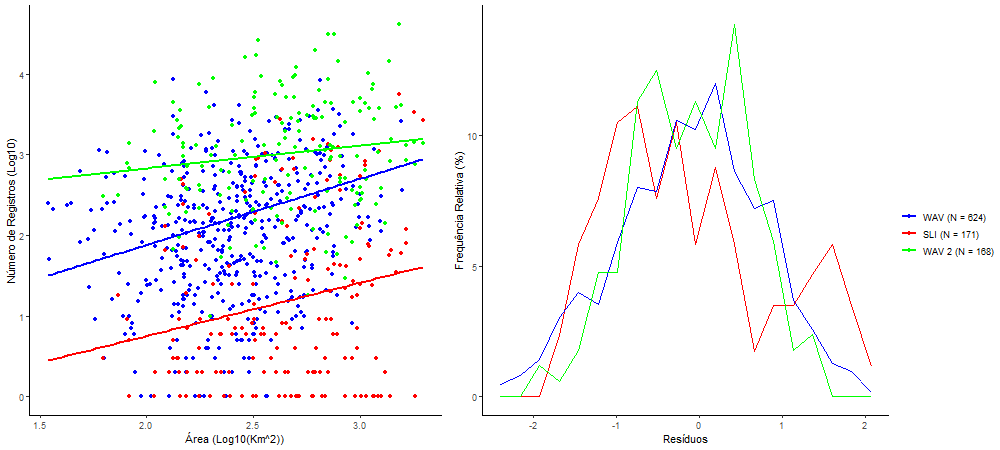
\includegraphics[width = 15cm]{Imagens/31213.png}
\\{\scriptsize Figura 10. Relação linear entre o número de registros (Log10) em cada banco de dados e a área (Log10 km2) dos municípios (esquerda) e respectiva distribuição de resíduos (direita, em unidades de desvio-padrão). Outliers bivariados foram excluídos.}
\end{figure}

\item População

\begin{figure}[h!]
\centering
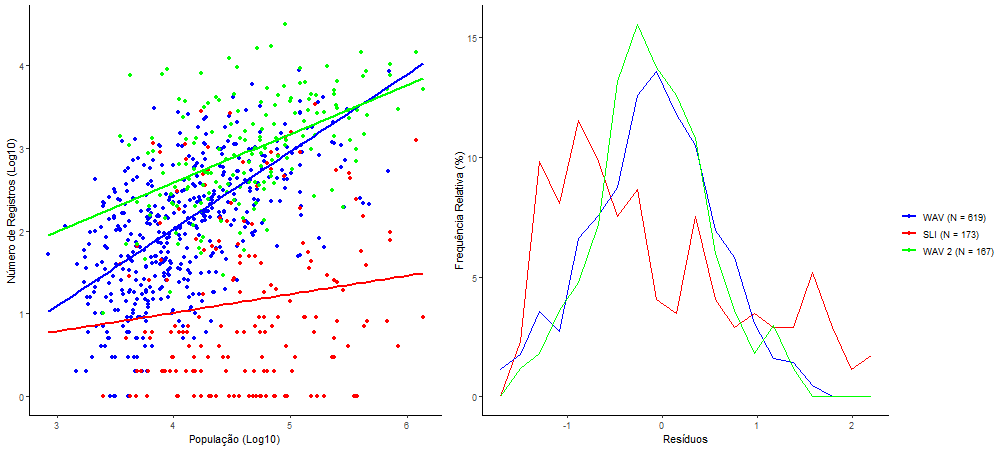
\includegraphics[width = 15cm]{Imagens/31313.png}
\\{\scriptsize Figura 11. Relação linear entre o número de registros (Log10) em cada banco de dados e o tamanho da população humana (Log10 indivíduos) dos municípios (esquerda) e respectiva distribuição de resíduos (direita, em unidades de desvio-padrão). Outliers bivariados foram excluídos.}
\end{figure}

\newpage

\item Latitude

\begin{figure}[h!]
\centering
\includegraphics[width = 15cm]{Imagens/31413.png}
\\{\scriptsize Figura 12. Relação linear entre o número de registros (Log10) em cada banco de dados e a latitude (graus) da sede dos municípios (esquerda) e respectiva distribuição de resíduos (direita, em unidades de desvio-padrão). Outliers bivariados foram excluídos.}
\end{figure}

\item Longitude

\begin{figure}[h!]
\centering
\includegraphics[width = 15cm]{Imagens/31513.png}
\\{\scriptsize Figura 13. Relação linear entre o número de registros (Log10) em cada banco de dados e a longitude (graus) da sede dos municípios (esquerda) e respectiva distribuição de resíduos (direita, em unidades de desvio-padrão). Outliers bivariados foram excluídos.}
\end{figure}

\newpage

\end{itemize}

\item Espécies

\begin{figure}[h!]
\centering
{\scriptsize Tabela 11: Correlação linear entre o número de espécies (Log10) por município em cada banco de dados e variáveis explanatórias. WAV = Wikiaves, SLI = SpeciesLink, WAV2 = WAV com municípios redundantes em SLI. Número de municípios (n), coeficiente de correlação de Pearson (r) para cada pareamento, com outliers bivariados excluídos. Valores significantes $(p < 0.05)$ em negrito.}
\\
\includegraphics[height = 10cm]{Tabelas/11.png}
\end{figure}

\begin{itemize}


\item Altitude

\begin{figure}[h!]
\centering
\includegraphics[width = 15cm]{Imagens/32113.png}
\\{\scriptsize Figura 14: Relação linear entre o número de espécies (Log10) em cada banco de dados e a altitude (m) da sede dos municípios (esquerda) e respectiva distribuição de resíduos (direita, em unidades de desvio-padrão). Outliers bivariados foram excluídos.}
\end{figure}



\item Área



\begin{figure}[h!]
\centering
\includegraphics[width = 15cm]{Imagens/32213.png}
\\{\scriptsize Figura 15: Relação linear entre o número de espécies (Log10) em cada banco de dados e a área (Log10 km2) dos municípios (esquerda) e respectiva distribuição de resíduos (direita, em unidades de desvio-padrão). Outliers bivariados foram excluídos.}
\end{figure}

\newpage

\item População

\begin{figure}[h!]
\centering
\includegraphics[width = 15cm]{Imagens/32313.png}
\\{\scriptsize Figura 16: Relação linear entre o número de espécies (Log10) em cada banco de dados e o tamanho da população humana (Log10 indivíduos) dos municípios (esquerda) e respectiva distribuição de resíduos (direita, em unidades de desvio-padrão). Outliers bivariados foram excluídos.}
\end{figure}


\item Latitude

 

\begin{figure}[h!]
\centering
\includegraphics[width = 15cm]{Imagens/32413.png}
\\{\scriptsize Figura 17: Relação linear entre o número de espécies (Log10) em cada banco de dados e a latitude (graus) da sede dos municípios (esquerda) e respectiva distribuição de resíduos (direita, em unidades de desvio-padrão). Outliers bivariados foram excluídos.}
\end{figure}

\newpage

\item Longitude

\begin{figure}[h!]
\centering
\includegraphics[width = 15cm]{Imagens/32513.png}
\\{\scriptsize Figura 18: Relação linear entre o número de espécies (Log10) em cada banco de dados e a longitude (graus) da sede dos municípios (esquerda) e respectiva distribuição de resíduos (direita, em unidades de desvio-padrão). Outliers bivariados foram excluídos.}
\end{figure}

\end{itemize}

\item Variáveis preditoras 

\begin{itemize}

\item Registros

\begin{figure}[h!]
\centering
\includegraphics[width = 12cm]{Imagens/4113.png}
\\{\scriptsize  Figura 19: Relação linear entre o número de registros (Log10) nos bancos de dados SLI e WAV2 pareados por X municípios redundantes e respectiva distribuição de resíduos (direita, em unidades de desvio-padrão). Outliers bivariados foram excluídos. n = 171, r2 = 0,1588, P $<$ 0,0001 .}
\end{figure}

\newpage

\item Espécies

\begin{figure}[h!]
\centering
\includegraphics[width = 12cm]{Imagens/4213.png}
\\{\scriptsize Figura 20: Relação linear entre o número de espécies (Log10) nos bancos de dados SLI e WAV2 pareados por X municípios redundantes e respectiva distribuição de resíduos (direita, em unidades de desvio-padrão). Outliers bivariados foram excluídos. n = 167 , r2 = 0,1523 , P $<$ 0,0001 .}
\end{figure}

\item Registros x Espécies

\begin{figure}[h!]
\centering
\includegraphics[width = 15cm]{Imagens/4333.png}
\\{\scriptsize Figura 21: Relação quadrática entre o número de espécies e o número de registros (ambos em Log10) nos bancos de dados WAV, SLI e WAV2 pareados por município e respectiva distribuição de resíduos (direita, em unidades de desvio-padrão). Outliers bivariados foram excluídos. n = 620, r2 = 0,9875, P $<$ 0,0001 no Wikiaves. n = 143, r2 = 0,9867, P $<$ 0,0001 no Wikiaves. n = 171, r2 = 0,9647, P $<$ 0,0001 no Wikiaves 2.}
\end{figure}

\end{itemize}

\item Distribuição Geográfica

\begin{figure}[h!]
\centering
\includegraphics[width = 10cm]{Imagens/511.png}
\\{\scriptsize Figura 22: Distribuição espacial dos municípios do estado de São Paulo em classes segundo a altitude (m) de sua sede.}
\end{figure}

\begin{figure}[h!]
\centering
\includegraphics[width = 10cm]{Imagens/521.png}
\\{\scriptsize Figura 23: Distribuição espacial dos municípios do estado de São Paulo em classes segundo a área (Log10 km2).}
\end{figure}

\begin{figure}[h!]
\centering
\includegraphics[width = 10cm]{Imagens/531.png}
\\{\scriptsize Figura 24: Distribuição espacial dos municípios do estado de São Paulo em classes segundo o tamanho da população humana (Log10 indivíduos).}
\end{figure}

\begin{figure}[h!]
\centering
\includegraphics[width = 15cm]{Imagens/561.png}
\\{\scriptsize Figura 25: Distribuição espacial dos municípios do estado de São Paulo em classes segundo o número de registros (Log10, esquerda) e o número de espécies (Log10, direita) em cada banco de dados (WAV = superior, SLI = central, WAV2 = inferior).}
\end{figure}

\end{itemize}

\newpage


\section{Conclusões e perspectivas de trabalhos futuros}

\input{Sections/07}

\bibliography{REF}


\end{document}
